Los algoritmos genéticos tienen cinco etapas
\begin{itemize}
    \item Definición de un individuo
    \item Creación de una población
    \item Medición del éxito de la población 
    \item Entrecruzamiento entre los mejores individuos para crear la siguiente generación
    \item Aplicación de mutaciones en los individuos de la nueva generación
\end{itemize}
A continuación veremos la aplicación de esas etapas en el problema propuesto, asumiendo que el $y_{critico}$ es conocido y es igual a $0$.
\[f(x,0)=x^{4}+0^{4}-x=f(x)=x^{4}-x\]\\
\framebreak
Para comenzar, iniciamos, proyectando la imagen de nuestra función de análisis:
    \begin{figure}[h]
       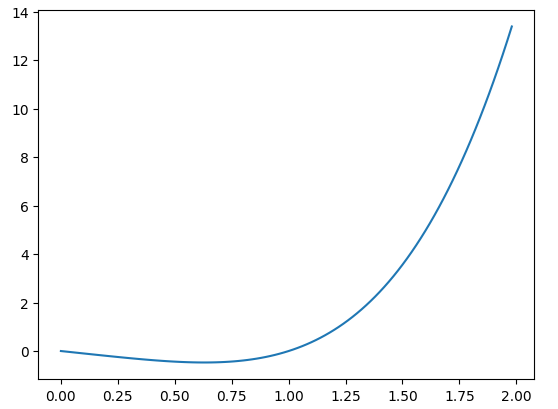
\includegraphics[width=6cm]{Imagenes/p3 ecuacion.png}
        \centering
    \end{figure}
Para este trabajo utilizamos un repositorio de GitHub con su aplicación para la maximización de funciones.\footcite{Dan20}
\framebreak

Generamos nuestra primera población:
    \begin{figure}[h]
       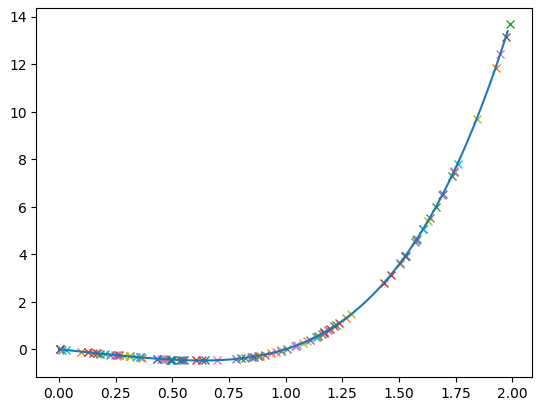
\includegraphics[width=6cm]{Imagenes/p3 1erag.png}
        \centering
    \end{figure}
A estos puntos los premiaremos cuando su valor sea mínimo y los castigaremos cuando el valor no cumpla con ese criterio, a esta evaluación se le conoce como "fitness"
\\
\framebreak
Luego de la primera generación, vemos que la distribución se ha movido ligeramente, pero no lo suficiente como para ser concluyente:
    \begin{figure}[h]
       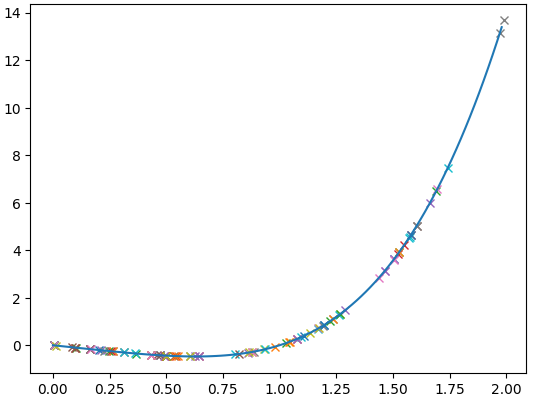
\includegraphics[width=6cm]{Imagenes/p3 2dag.png}
        \centering
    \end{figure}
Hay que resaltar que en todas las generaciones se aplicó una mutación, es decir, se vario uno de los genes de algunos individuos de manera aleatoria.
\\
\framebreak
Luego de 100 generaciones, la población se ha distribuido de la siguiente manera:
    \begin{figure}[h]
       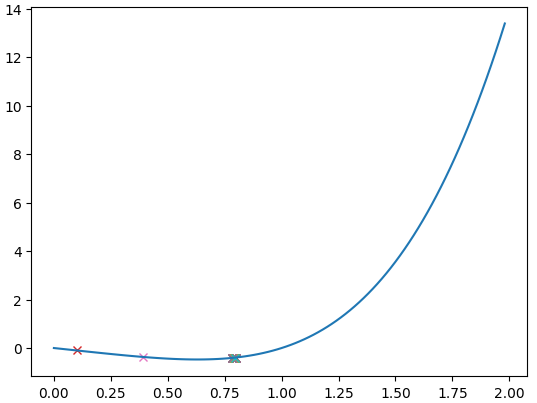
\includegraphics[width=6cm]{Imagenes/p3 100g.png}
        \centering
    \end{figure}
El valor de $x$ que arroja el mínimo en esta función ha sido $x=0.796$, un valor cercano al valor calculado, pero como hemos podido observar, luego de una determinada cantidad de generaciones, seguramente será posible obtener un valor más cercano al valor calculado analíticamente.
\\Si queremos seguir generando poblaciones, podemos utilizar el siguiente enlace hecho en Google Coolab para esta función: \href{https://colab.research.google.com/drive/1-Qyot1mxXB_5UUK7yPKAN7h3VYBSTotL#scrollTo=u9t-hjTo2aWS}{Enlace de Coolab}
